%%%%%%%%%%%%%%%%%%%%%%%%%%%%%%%%%%%%%%%%%%%%%%%%%%%%%%%%%%%%
%%  This Beamer template was created by Cameron Bracken.
%%  Anyone can freely use or modify it for any purpose
%%  without attribution.
%%
%%  Last Modified: January 9, 2009
%%

\documentclass[xcolor=x11names,compress]{beamer}

%% General document %%%%%%%%%%%%%%%%%%%%%%%%%%%%%%%%%%
\usepackage{epstopdf}
\usepackage{graphicx}
\usepackage{tikz}
\usepackage[french]{babel}
\usepackage[T1]{fontenc}
\usepackage[utf8]{inputenc}
\usepackage{array}
\usepackage{svg}
\usepackage{calc}
\usetikzlibrary{decorations.fractals, calc}
%%%%%%%%%%%%%%%%%%%%%%%%%%%%%%%%%%%%%%%%%%%%%%%%%%%%%%


%% Beamer Layout %%%%%%%%%%%%%%%%%%%%%%%%%%%%%%%%%%
\mode<presentation> {
  \usetheme{CustomTheme}
}
%%%%%%%%%%%%%%%%%%%%%%%%%%%%%%%%%%%%%%%%%%%%%%%%%%

\setbeamercovered{invisible}

\AtBeginSection[]{%
  \begin{frame}<beamer>
  \tableofcontents[currentsection]
  \end{frame}
}


\begin{document}


%%%%%%%%%%%%%%%%%%%%%%%%%%%%%%%%%%%%%%%%%%%%%%%%%%%%%%
%%%%%%%%%%%%%%%%%%%%%%%%%%%%%%%%%%%%%%%%%%%%%%%%%%%%%%
\begin{frame}
\title{Développement, amélioration et intégration d'outils de génération de code}
\subtitle{pour une plateforme de prototypage de fonctions de contrôle moteur.}
\author{
  \vspace{-15px}\\
  Mathieu {\sc Soum}\\
  {\footnotesize
    Université Paul Sabatier\\
    \vspace{-1px}
    Master 2 -- Développement Logiciel\\
  }
  \vspace{5px}
  {\small Stage réalisé chez Aboard Engineering}\\
  {\scriptsize
    Maître de stage : Sébastien {\sc Riche}\\
    \vspace{-5px}
    Tutrice universitaire : Isabelle {\sc Ferrané}
  }
  \vspace{-17px}
}
\date{
	{
	  \begin{tabular}{m{90pt}m{105pt}m{85pt}}
		
\includegraphics[scale=0.20]{images/aboard} &
		
\includegraphics[scale=0.1]{images/mdl} &
		
\includegraphics[scale=0.25]{images/ups} \\
	  \end{tabular}
	  %
\includegraphics[scale=0.4]{images/aboard}\hspace{75px}
\includegraphics[scale=0.37]{images/ups}
	}
	\\
	\vspace{5px}
	Année universitaire 2014 - 2015
}
\titlepage
\end{frame}

%%%%%%%%%%%%%%%%%%%%%%%%%%%%%%%%%%%%%%%%%%%%%%%%%%%%%%
%%%%%%%%%%%%%%%%%%%%%%%%%%%%%%%%%%%%%%%%%%%%%%%%%%%%%%
\section{\scshape Contexte}
\begin{frame}{\vspace{-17pt}\\
\includegraphics[scale=0.25]{images/aboard}}
  \begin{center}
	{\footnotesize Automobile, Aéronautique, Marine, Loisir, Industriel de la
	R\&D à la série}\\
	\vspace{10pt}
	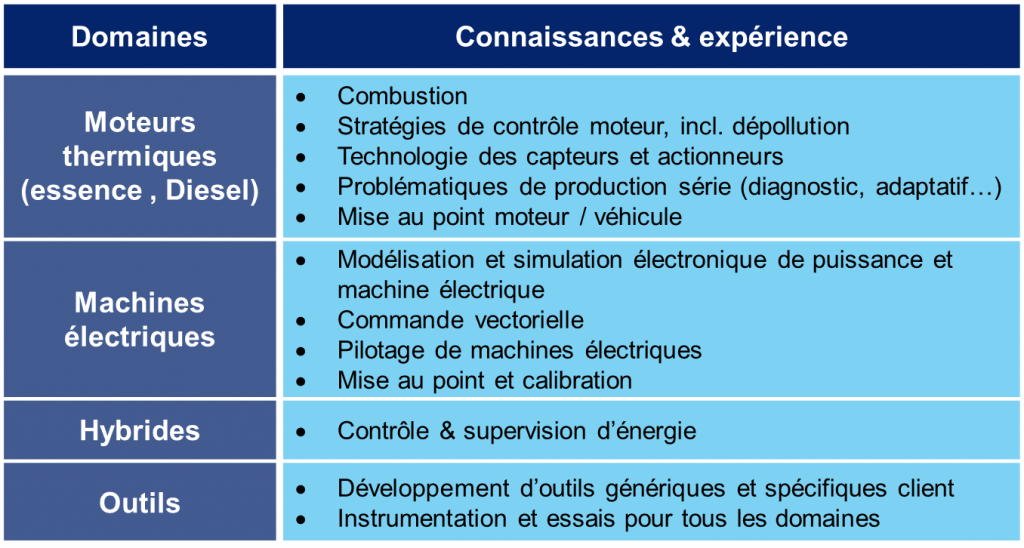
\includegraphics[scale=0.3]{images/domaines}\\
  \end{center}
\end{frame}

%%%%%%%%%%%%%%%%%%%%%%%%%%%%%%%%%%%%%%%%%%%%%%%%%%%%%%
%%%%%%%%%%%%%%%%%%%%%%%%%%%%%%%%%%%%%%%%%%%%%%%%%%%%%%
\section{\scshape Objectifs}
\begin{frame}{\vspace{-17pt}\\
\includegraphics[scale=0.4]{images/orianne}}
  \begin{center}
	\onslide<1->{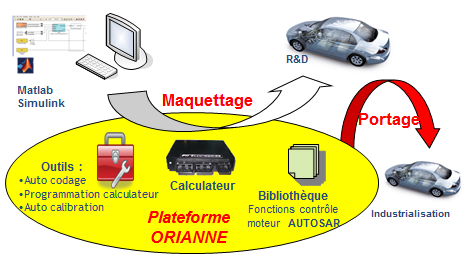
\includegraphics[scale=0.6]{images/orianne_schema}}
	\vfill
	\onslide<2->{
	  \begin{tabular}[h]{m{110pt}m{53pt}m{125pt}}
	  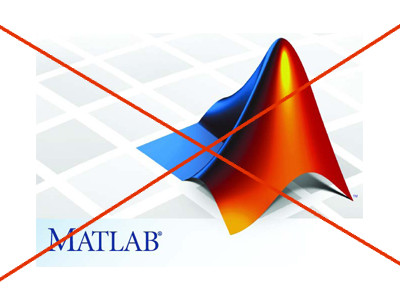
\includegraphics[scale=0.25]{images/matlablogo_cross} &
	  
\includegraphics[scale=2.5]{images/rightarrow.eps} &
	  
\includegraphics[scale=0.1]{images/qgen} \\
	  \end{tabular}
	}
  \end{center}
\end{frame}

\begin{frame}{\vspace{-17pt}\\
\includegraphics[scale=0.05]{images/qgen}}
  \begin{center}
	Générateur de code embarqué C/Ada depuis Matlab Simulink.\\
	\vfill
	\begin{tabular}[h]{m{150pt}m{150pt}}
	  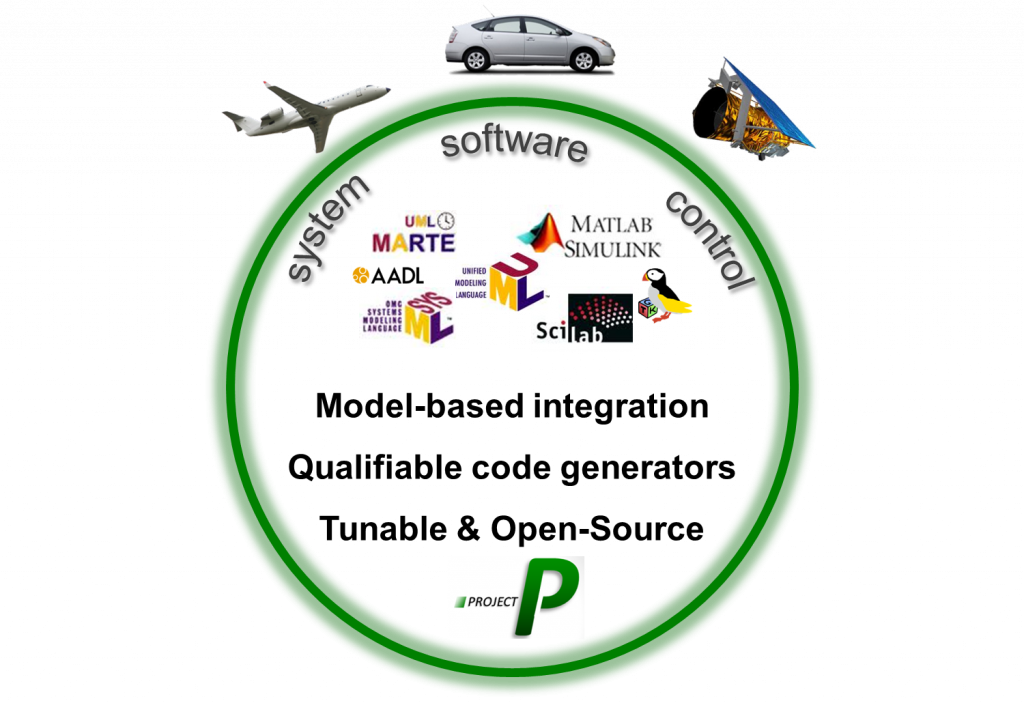
\includegraphics[scale=0.14]{images/projectp}&
	  
\includegraphics[scale=0.24]{images/adacore.png}\\
	\end{tabular}
	\vfill
	\begin{block}{Avantages}{}
	  \begin{itemize}
		\item Prix
		\item Maîtrise
	  \end{itemize}
	\end{block}
  \end{center}
\end{frame}

\begin{frame}{\vspace{-17pt}\\
\includegraphics[scale=0.4]{images/orianne}}
  \centering
  \og coopération sur les standards,\\
  concurrence sur la mise en \oe uvre \fg{}
  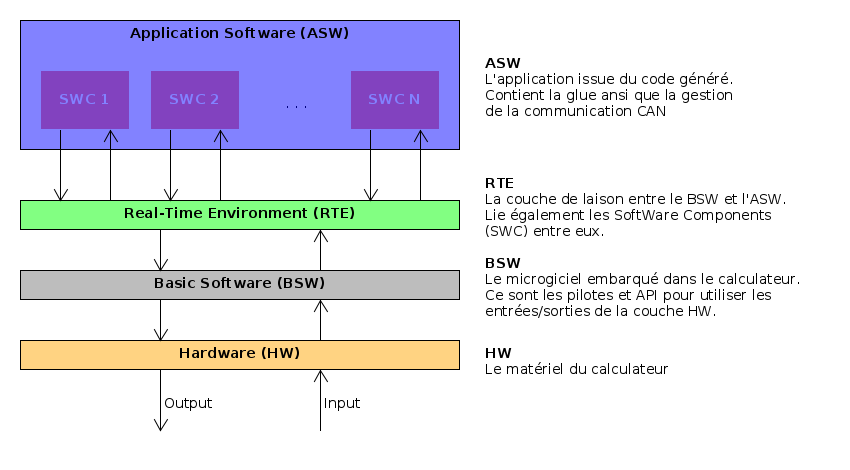
\includegraphics[scale=0.37]{images/autosar_arch}
\end{frame}

\begin{frame}{{\bf C}ontroller {\bf A}rea {\bf N}etwork}
  \begin{center}
	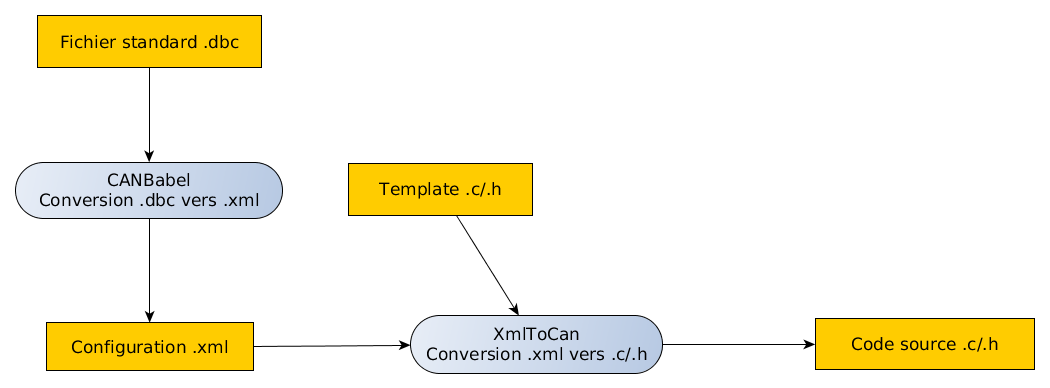
\includegraphics[scale=0.28]{images/dbctocan}\\
	\vfill
	Processus de convertion des fichiers .dbc vers du code source C
  \end{center}
\end{frame}

\begin{frame}{Objectifs}
  \begin{block}{QGen}{}
	\begin{itemize}
	  \item Analyse du code
	  \item Identification des problèmes
	  \item Collaboration avec AdaCore
	\end{itemize}
  \end{block}
  \begin{block}{Plateforme Orianne}{}
	\begin{itemize}
	  \item Génération CAN fonctionnelle et viable
	  \item Intégration à l'IHM Orianne
	  \item Conception des outils manquants
	\end{itemize}
  \end{block}
\end{frame}

%%%%%%%%%%%%%%%%%%%%%%%%%%%%%%%%%%%%%%%%%%%%%%%%%%%%%%
%%%%%%%%%%%%%%%%%%%%%%%%%%%%%%%%%%%%%%%%%%%%%%%%%%%%%%
\section{\scshape Travail réalisé}
\begin{frame}{QGen -- Analyse}
  \vfill
  Analyse statique (OCLint)
  \begin{itemize}
	\item Complexité
	\item Propreté du code
  \end{itemize}
  \vfill
  Analyse à l'execution
  \begin{itemize}
	\item Espace de stockage
	\item Mémoire
	\item Temps d'execution
  \end{itemize}
  \vfill
\end{frame}

\begin{frame}{QGen -- Premiers résultats}
  \vfill
  Analyse statique : codes équivalents\\
  \vfill
  Analyse à l'exécution :
  \begin{itemize}
	\item Moins performant
	\item Plus volumineux
  \end{itemize}
  \vfill
  \centering
  {\bf Facteur 2}
  \vfill
\end{frame}

\begin{frame}{QGen -- Hypothèses d'améliorations}
  \vfill
  \begin{itemize}
	\item Extrapolation et interpolation
	\item Variables intermédiaires
	\item Déclaration des entrée/sorties
  \end{itemize}
  \vfill
\end{frame}

\begin{frame}{QGen -- Dernières métriques}
  \vfill
  Résultats équivalents entre QGen et Matlab RTW-EC.
  \begin{itemize}
	\item Temps d'execution : $800\mu s$ $\Rightarrow$ $400\mu s$
	\item Espace de stockage grandement diminué
  \end{itemize}
  \vfill
  \centering
  Résultats très concluants\\
  Première version majeure annoncée
  \vfill
\end{frame}


\begin{frame}{Orianne -- Découverte de la plateforme}
  \vfill
  Architecture : Composants OSGi
  \begin{alertblock}{Non pertinent}{}
	\begin{itemize}
	  \item Manque de modularité
	  \item Redondance
	  \item Linéarité
	\end{itemize}
  \end{alertblock}
  \vfill
  \centering
  {\Huge $\rightarrow$} 
\includegraphics[scale=0.25]{images/maven.png}
  \vfill
\end{frame}

\begin{frame}{Orianne -- Générateur CAN}
  Trop de mémoire utilisée $\Rightarrow$ code inutilisable
  \vfill
  Étude de l'existant :
  \begin{itemize}
	\item Redondance
	\item Linéarité
	\item Complexité
  \end{itemize}
  \vfill
  \centering
  Factorisation, abstraction $\Rightarrow$ Clarté, maintenabilité
  \vfill
\end{frame}

\begin{frame}{Orianne -- Générateur CAN}
  Adaptation des templates
  \begin{itemize}
	\item Suppression des données inutilisées
	\item Passage en constante des configurations
	\item Factorisation du code généré
  \end{itemize}
\end{frame}

\begin{frame}{Orianne -- Intégration à l'IHM}
  \centering
  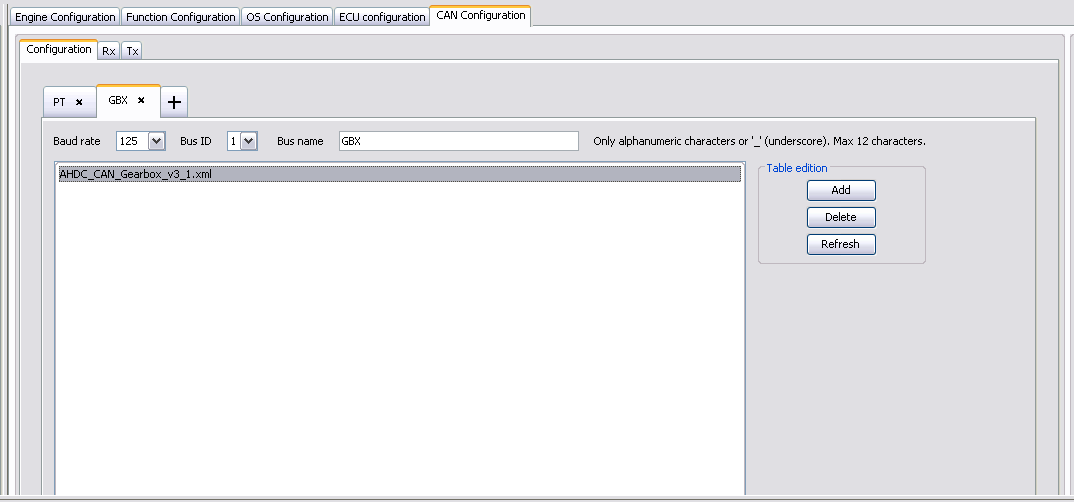
\includegraphics[scale=0.3]{images/ihmcan_conf}
\end{frame}

\begin{frame}{Orianne -- Intégration à l'IHM}
  \centering
  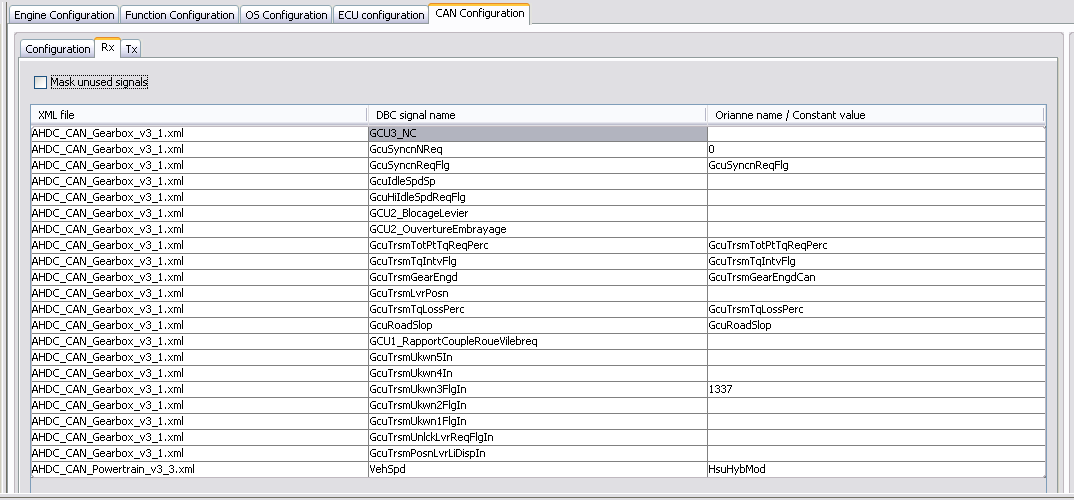
\includegraphics[scale=0.3]{images/ihmcan_signal}
\end{frame}

\begin{frame}{Orianne -- Bilan CAN}
  Objectif de performance atteint
  \begin{center}
	{\large {\bf Facteur 7}}
  \end{center}
  Code généré testé et validé\\
  \vfill
  IHM de configuration complète
\end{frame}

\begin{frame}{Orianne -- Partie RTE}
  \centering
  \vfill
  Configuration complète via l'IHM\\
  Développement du générateur
  \vfill
\end{frame}

%%%%%%%%%%%%%%%%%%%%%%%%%%%%%%%%%%%%%%%%%%%%%%%%%%%%%%
%%%%%%%%%%%%%%%%%%%%%%%%%%%%%%%%%%%%%%%%%%%%%%%%%%%%%%
\section{\scshape Bilan}
\begin{frame}{Expérience professionnelle}
  \vfill
  \begin{itemize}
	\item Découverte du domaine automobile
	\item Expérience en alternance
	\item Atteinte des objectifs
  \end{itemize}
  \vfill
\end{frame}

\begin{frame}{Apports personnels}
  \vfill
  \begin{itemize}
	\item Intérêt pour l'informatique embarquée
	\item Approfondissement technique
	\item Confort de mes compétences en anglais
  \end{itemize}
  \vfill
\end{frame}

%%%%%%%%%%%%%%%%%%%%%%%%%%%%%%%%%%%%%%%%%%%%%%%%%%%%%%
%%%%%%%%%%%%%%%%%%%%%%%%%%%%%%%%%%%%%%%%%%%%%%%%%%%%%%
\section*{}
\begin{frame}
\title{Développement, amélioration et intégration d'outils de génération de code}
\subtitle{pour une plateforme de prototypage de fonctions de contrôle moteur.}
\author{
  \vspace{-15px}\\
  Mathieu {\sc Soum}\\
  {\footnotesize
    Université Paul Sabatier\\
    \vspace{-1px}
    Master 2 -- Développement Logiciel\\
  }
  \vspace{5px}
  {\small Stage réalisé chez Aboard Engineering}\\
  {\scriptsize
    Maître de stage : Sébastien {\sc Riche}\\
    \vspace{-5px}
    Tutrice universitaire : Isabelle {\sc Ferrané}
  }
  \vspace{-17px}
}
\date{
	{
	  \begin{tabular}{m{90pt}m{105pt}m{85pt}}
		
\includegraphics[scale=0.20]{images/aboard} &
		
\includegraphics[scale=0.1]{images/mdl} &
		
\includegraphics[scale=0.25]{images/ups} \\
	  \end{tabular}
	  %
\includegraphics[scale=0.4]{images/aboard}\hspace{75px}
\includegraphics[scale=0.37]{images/ups}
	}
	\\
	\vspace{5px}
	Année universitaire 2014 - 2015
}
  \titlepage
\end{frame}

\begin{frame}{AUTOSAR}
  \centering
  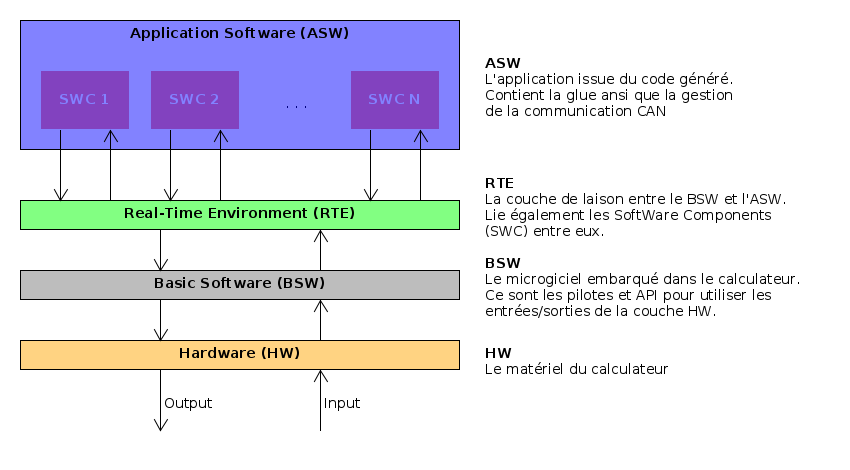
\includegraphics[scale=0.40]{images/autosar_arch}
\end{frame}

\end{document}
